\documentclass{article}
\usepackage[spanish]{babel}
\usepackage[numbers,sort&compress]{natbib}
\usepackage[T1]{fontenc}
\usepackage[ansinew]{inputenc}
\usepackage{graphicx}
\usepackage{url}
\usepackage{caption}
\usepackage{float}
\usepackage{subcaption}
\usepackage{caption}
\usepackage{listings}
\usepackage{amsmath}
\usepackage{natbib}
\usepackage[numbers,sort&compress]{natbib}

\title {Modelo de Urnas}
\author{Oscar Qui\~nonez}

\begin{document}

\maketitle
 
\section{Objetivo}\label{met}

Se busca representar la fragmentaci\'on y la uni\'on de part\'iculas, que al unirse forman mol\'eculas m\'as grandes que se denominaran c\'umulos, estos a su vez se pueden volver a fragmentar, por lo tanto, se intenta calcular el porcentaje de c\'umulos que podr\'ian pasar a trav\'es de un filtro debido su tama\~no \cite{satuelisa}.

\section{Metodolog\'ia}\label{met}

Para lograr la simulaci\'on del filtrado de las part\'iculas, es necesario el uso del software Python 3.7, en el que se toma como base el c\'odigo \cite{doctora} para representar variaciones en el n\'umero de c\'umulos (k), al n\'umero de part\'iculas (n) y tambi\'en al n\'umero de pasos (t) \cite{discord}. A partir de los n\'umeros colocados en una lista se le da valor a  (c) como tama\~no critico del filtro, por lo que, s\'i el valor del c\'umulo es mayor, ser\'a parte de los filtrados y si es menor, permanecer\'a en los no filtrados.
Los valores de k son: 1000, 2500, 5000, 7500 y 10000; los valores en n son: 100000, 500000 y 1000000; mientras que los valores de t son: 20, 40, 60, 80 y 100.

\section{Resultados y Discusi\'on}\label{res}

Despu\'es de procesar los datos en el c\'odigo, se obtuvo una gr\'afica para un valor de t, por lo que fue necesario correr el c\'odigo 5 veces, una para cada valor. Las gr\'aficas que se muestran a continuaci\'on como figura 1 son de tipo caja-bigote y nos sirven para representar los valores promedio del porcentaje de filtraci\'on, para t=20 los valores de 1000, 2500, 5000, 7500 y 10000 fueron aproximadamente de 25, 12, 8, 135 y 38 respectivamente; para el resto de los valores en t (40, 60, 80 y 100) se obtuvieron promedios muy similares como se pueden apreciar al comparar las gr\'aficas, esto nos indica que k=7500 se obtuvo el mayor porcentaje de filtraci\'on pues se acerca 140 en las 5 gr\'aficas \cite{yo}.

\begin{figure}
       \centering
       \begin{subfigure}[b]{0.49\linewidth}
           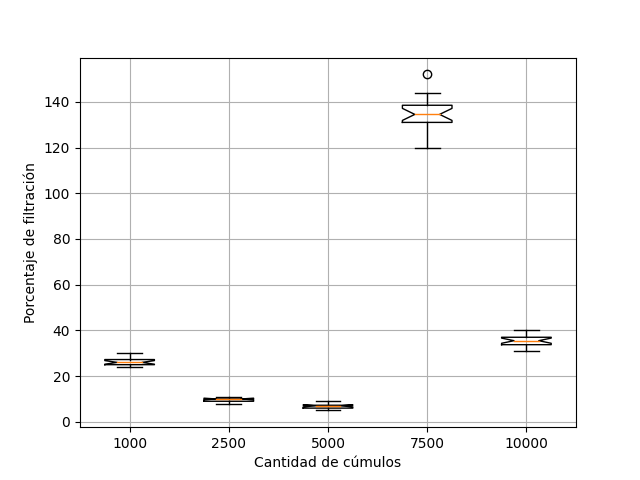
\includegraphics[width=\linewidth]{tareaocho20.png}
           \caption{t=20}
           \label{fig:westminster_lateral}
        \end{subfigure}
        \begin{subfigure}[b]{0.49\linewidth}
            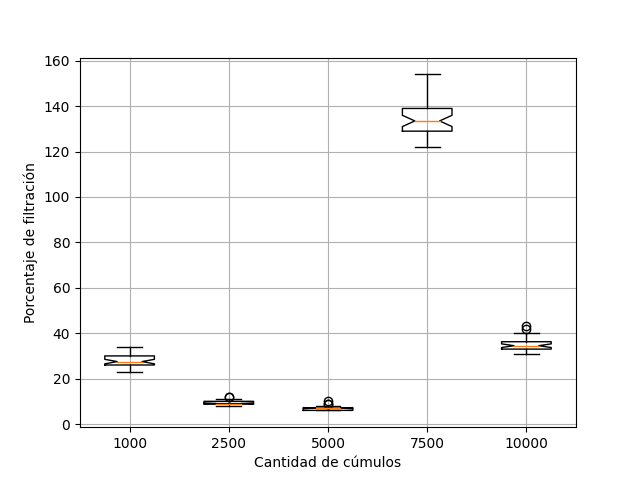
\includegraphics[width=\linewidth]{tareaocho40.png}
            \caption{t=40}
            \label{fig:westminster_aerea}
        \end{subfigure}
        \begin{subfigure}[b]{0.49\linewidth}
            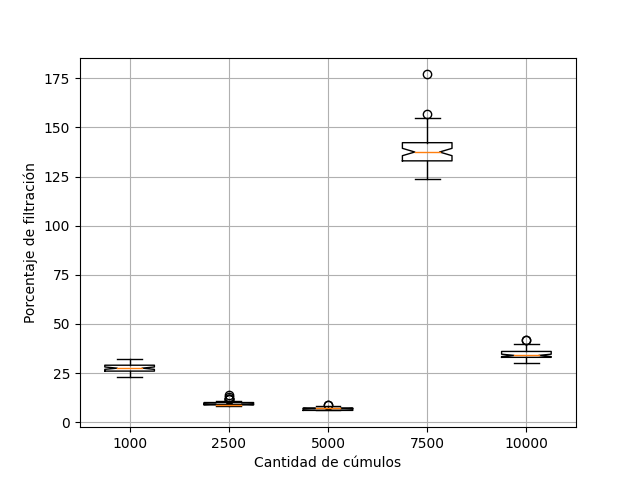
\includegraphics[width=\linewidth]{tareaocho60.png}
            \caption{t=60}
            \label{fig:westminster_aerea}
        \end{subfigure}
        \begin{subfigure}[b]{0.49\linewidth}
            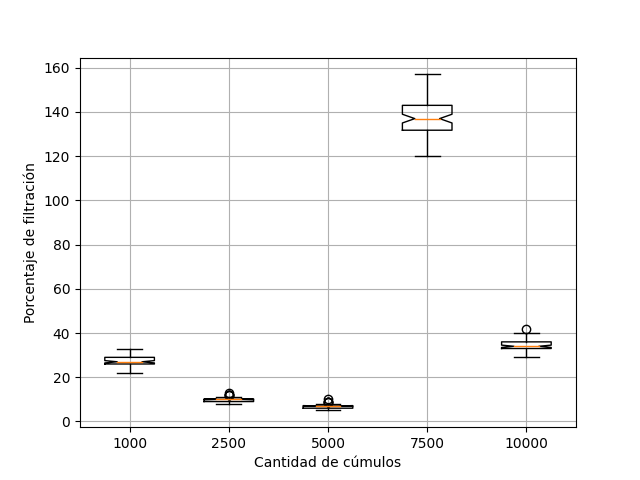
\includegraphics[width=\linewidth]{tareaocho80.png}
            \caption{t=80}
            \label{fig:westminster_aerea}
        \end{subfigure}
        \begin{subfigure}[b]{0.49\linewidth}
            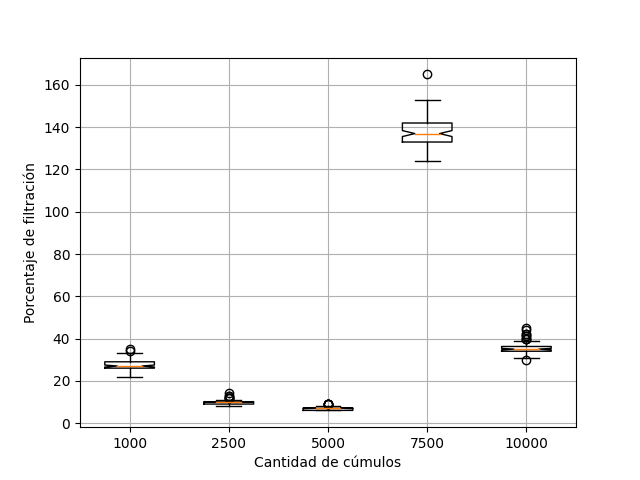
\includegraphics[width=\linewidth]{tareaocho100.png}
            \caption{t=100}
            \label{fig:westminster_aerea}
        \end{subfigure}
        \caption{Gr\'aficas obtenidas para diferentes valores en t.}
        \label{fig:westminster}
\end{figure}

\section{Conclusi\'on}

Cuando se incrementa los valores del tama\~no de part\'icula, van generando una gran cantidad de c\'umulos lo que provoca una menor cantidad de filtrados, sin embargo, en 7500 no pasa esto, pues es notable la diferencia en la gr\'afica, lo que se atribuye a que el valor alcanza un punto en donde es menor al critico y luego vuelve a decrecer en 10000.

\bibliography{tareaocho}
\bibliographystyle{unsrtnat}

\end{document}
